\section{Methods: the verified foundation layer}\label{sec:methods}

Natural units, $c = 1$. The foundation modules were checked for numerical
correctness against known results (sprinkling measure, Minkowski causal
precedence, longest-chain and interval-cardinality normalizations,
Myrheim--Meyer inversion, radar/Lorentz/Rindler formulas); this section
states the conventions the results depend on. \Fref{fig:setup} illustrates
the primitive and two of the operational constructions.

\begin{figure}[t]
\centering
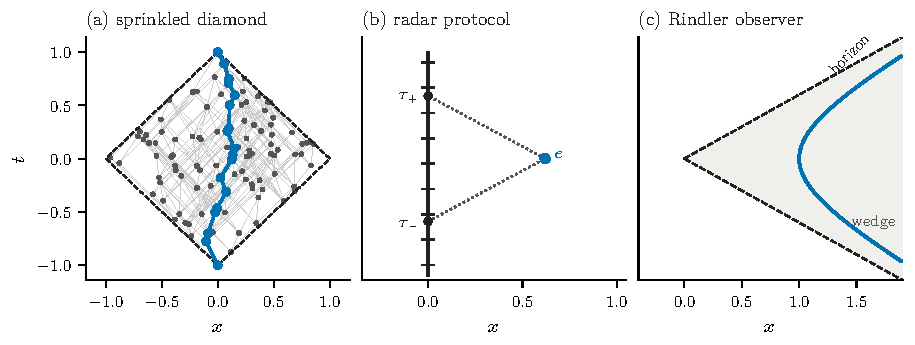
\includegraphics[width=\textwidth]{figures/fig0_setup.pdf}
\caption{The primitive and two operational constructions (illustrations
drawn with the foundation modules at a fixed seed; no measured quantity is
displayed). (a)~A Poisson sprinkling into a $(1{+}1)$D causal diamond, with
its covering (Hasse) relations in gray and one longest chain between the
diamond tips highlighted. (b)~The radar protocol: an observer chain with
tick labels, and the latest preceding ($\tau_-$) and earliest succeeding
($\tau_+$) ticks that bound a target event $e$. (c)~An accelerated
(Rindler) observer's worldline; its two-way radar reconstruction is
confined to the shaded wedge, whose boundary is the horizon.}
\label{fig:setup}
\end{figure}

\begin{itemize}
\item \textbf{Sprinkling.} Events are sampled uniformly with respect to the
  Minkowski volume in a causal diamond (rejection sampling on the
  ball-volume slice; equivalently uniform in null coordinates). The
  $(1{+}1)$D and $D$-dimensional diamonds and the $(1{+}1)$D forward cone
  are provided.
\item \textbf{Causal order.} For events $(t, x)$, $i$ precedes $j$ iff
  $t_j - t_i > 0$ and $(t_j - t_i)^2 - |x_j - x_i|^2 \ge -\texttt{atol}$
  (null-inclusive $J^+$; strict in time, so irreflexive).
\item \textbf{Longest chain.} Topological-sort longest-path dynamic
  programming on the order; the $(1{+}1)$D proper-time normalization uses
  the Brightwell--Gregory constant ($L \sim \sqrt{2\rho}\,\tau$, i.e.\
  $L \sim 2\sqrt{N}$ in a diamond of $N$ events, consistent with
  \sref{sec:r1} and appendix~\ref{app:conventions}), with an
  endpoint-inclusive counting convention and acknowledged finite-size
  corrections.
\item \textbf{Interval cardinality.} The open Alexandrov interval count $K$
  between two events estimates volume $V = K/\rho$; in $(1{+}1)$D
  $V = \tau^2/2$, so $\tau_{\mathrm{est}} = \sqrt{2K/\rho}$.
\item \textbf{Myrheim--Meyer dimension.} The ordering fraction (related
  pairs over all pairs) is inverted against the known $f(d)$ curve to
  estimate spacetime dimension in flat Alexandrov intervals.
\item \textbf{Radar coordinates.} For a supplied observer chain, $\tau_-$
  and $\tau_+$ are the latest preceding and earliest succeeding tick
  labels; radar time is their mean and radar distance their
  half-difference. A single chain gives unsigned distance; a second
  oriented chain supplies the sign. Lorentz maps between two inertial
  protocols are fit on their overlap \cite{perlick2008}.
\item \textbf{Rindler.} An accelerated (Rindler) observer in flat
  spacetime, with analytic two-way radar ticks; the reconstructible region
  is the Rindler wedge, with the horizon appearing as a
  reconstruction-inaccessibility boundary \cite{rindler1966}.
\item \textbf{Conformal / measure.} Positive conformal rescalings preserve
  causal order while changing volume and clock scale; volume reconstruction
  then requires supplied measure information (implemented in \expid{exp19}
  as local weights). In the tested random-thinning protocol, reconstruction
  is stable after density rescaling.
\end{itemize}
